\section{Measures}
\label{sec:measures}
\subsection{Qualitative Measures}
In order to collect the parents' and children's opinions on the interaction, we conducted interviews after each session.
These interviews aimed to collect data on acceptability, trust and credibility and to do a comparison between conditions and between parents and children>

Building an interview that would suit both parents and children was a hard task\footnote{Interviews and Questionnaire used are available online: }.%todo put online



The last part questionnaire, after the second session, is based on the Godspeed\cite{Bartneck2008b} items about Credibility, Likeability and Complicity.
We also used the COIRS~\cite{Robert2014} questionnaire and adapted it for the parents.
After each session, the parents and the children would reply to the interview; and after the second a final interview would deal with explicit comparison of the two sessions by the participants.


In addition to these qualitative evaluations at the end of the last session, the participants are asked to reply to a final survey in which they compare the conditions directly.
This allows us to obtain the participants' preferences and to see if it is correlated to other measures.

\subsection{Quantitative Measures}
Objective measures are also collected to evaluate variations in the performance of children at the math test, and the attitude in the different tasks using the Kinect Sensor.

The attitude analysis is computed from skeleton data.
We base our quantitative analysis body measures defined in the Psychology literature.
This analysis will allow us to compare behaviour of the child according to the robot's style in front of him and to the versatility of the robot.

\subsection{Data capture}
\begin{figure}[h]
	\begin{tabular}{|c | c|}
		\hline
		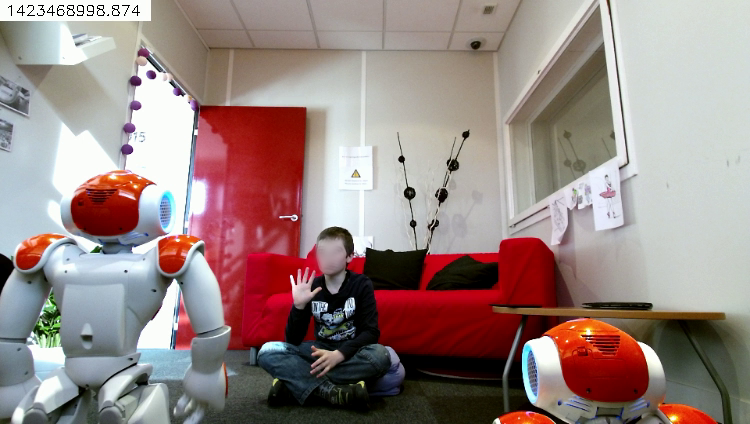
\includegraphics[width=0.45\columnwidth]{Figures/illustrate/k2a}&
		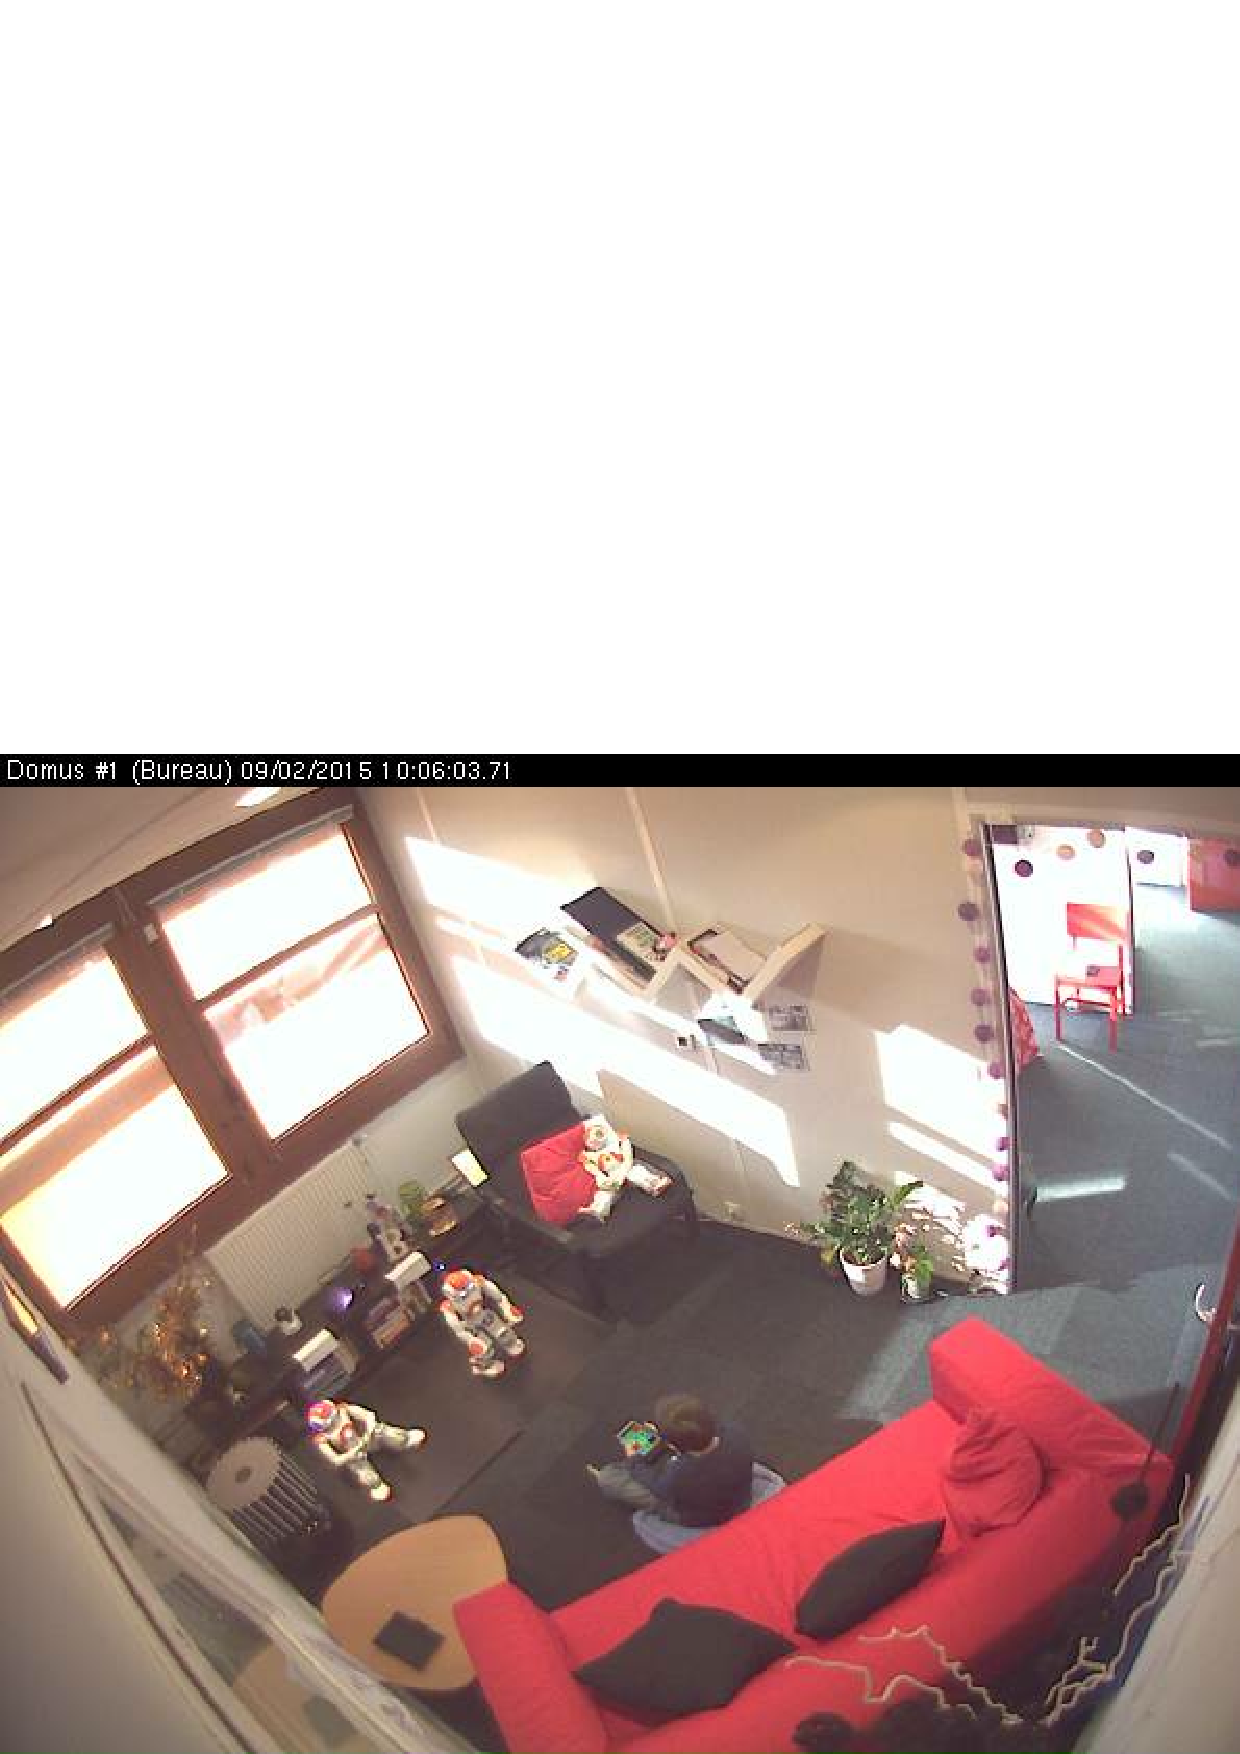
\includegraphics[width=0.45\columnwidth]{Figures/illustrate/ceilingb1}\\
		Image from video capture from Kinect View &
		Ceiling Back View \\\hline
		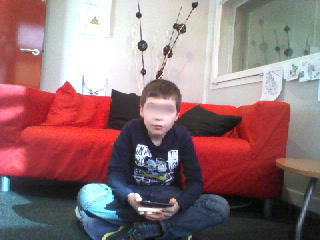
\includegraphics[width=0.45\columnwidth]{Figures/illustrate/robotview}&
		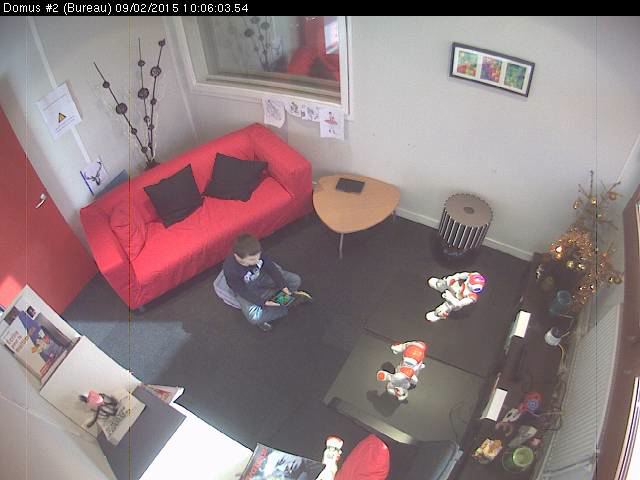
\includegraphics[width=0.45\columnwidth]{Figures/illustrate/ceilingf1}\\
		Robot's Camera View &
		Ceiling Front View\\ \hline
	\end{tabular}
	\caption{Samples of Video captures from the 4 cameras in the experiment}
	\label{fig:allcam}
\end{figure}

In order to be able to analyse the impact of the robot's style on the child's behaviour, we used a Kinect sensor and recorded all the available channels.
It was a Kinect Sensor 2 from Microsoft.

We used a program developed for MobileRGB-D to record raw data from the Kinect at a frame rate of 30FPS~\cite{MobileRGB}.
Two video cameras in the ceiling (Fig. \ref{fig:allcam})  were also recording the interaction and were allowing the parents to see the interaction live in the control room.
The robot was recording logs of the interaction with the tablet (question, answers and timestamps) that were after used to label the activities  automatically.
We also recorded videos from the robots' cameras.
For one of the children, a GoPro camera was also used to have images of the child's point of view during the interaction (Fig. \ref{fig:gopro2}).



%
%The recorded data is summarised in table \ref{tab:dataset}
%\begin{table}[h]
%	\centering
%	\caption{Data recorded during the interaction with the robots}
%
%	\begin{tabular}{p{1cm} p{1.5cm} p{1.5cm} p{2.5cm}}
%		\hline
%		Data  & Sensor & Frequency & \\ \hline
%		RGB Video & Microsoft Kinect 2 & 30 Hz max & Resolution 1900*1080p \\
%		Depth & Microsoft Kinect 2 & 30 Hz max & Resolution 512*424p from 40cm to 4.5m \\
%		Body & Microsoft Kinect 2 & 30 Hz max & 6 bodies maximum with 25 joints (3D positions and 3D orientations as quaternions)\\
%		Infrared & Microsoft Kinect 2 & 30 Hz & Resolution 512*424p \\
%		Audio & Microsoft Kinect 2 &  &  \\
%		\hline
%		Video & Ceiling Office 1 \& 2 & $<$ 30 Hz & Resolution 640*480 \\
%		\hline
%		Video & Nao Robot 1 & 15 Hz & Resolution 320*480 \\
%		Video & Nao Robot 2 & 15 Hz & Resolution 320*480 \\
%		\hline
%	\end{tabular}
%	\label{tab:dataset}
%\end{table}


Every session was about 250Gb of recorded data on the disk.
In total, we have collected about 8To of data.
We present in this paper only the body analysis data that constitute one of our contribution.


\subsection{Measures Extracted from Body Analysis}
We used the skeleton data to measure variation on the child's attitude between the sessions.
Several features form the literature of body communication have been implemented and applied for the Body Kinect data \cite{larboulette2015review}.

\subsubsection{Static Features}
We first extracted static body features at every frame:
\begin{itemize}[noitemsep,nolistsep]
\item \textbf{Body Volume}: Bounding box of the skeleton data
\item \textbf{Center of Mass}: Position in 3D coordinates of the centre of mass
\item \textbf{Center of Mass Displacement}: Variation of Position in 3D coordinates of the centre of mass from one frame to the next
\item \textbf{Distance/area Covered}: measures the area covered by the projection of the COM on the floor over a time period
\item \textbf{Hand Relationship}: 3D distance between hands
\item \textbf{Shoulder Angle}: rotation angle of shoulders according to the torso vertical axis
\item \textbf{Elbow Flexion}: aperture angle of the elbow joints
\item \textbf{Feet Relationship}: 3D distance between feet
\item \textbf{Torso Neck Orientation}: %todo
\item \textbf{Hands Status}: open or closed
\end{itemize}

\paragraph{Volume}
For each frame, the volume is computed by going through the joints and recording the min and max in all three dimensions (X,Y,Z).
We also use as feature the joint's name at the minimum and the maximum for all three dimensions.

\paragraph{Center of Mass}

\paragraph{Leaning angle}
Leaning left and right corresponds sideways lean (see Fig. \ref{fig:sideways_lean}), while leaning forward and back corresponds to frontal leaning angle (see Fig. \ref{fig:BLA}).
The values range between $-1$ and $1$ in both directions, where 1 roughly corresponds to $45\deg$ of lean.

In addition to the given angles from the Kinect sensor for the leaning angles, we computed a body lean angle in line with the work of \cite{Castellano2009} and \cite{Schegloff}. This angle, was computed by the dot product of the vertical vector from the hip centre joint and the vector from the hip centre to the shoulder centre of each collected body data frame.

\paragraph{Torso and Neck Orientations}
TorsoQ and NeckQ are given by the Kinect sensor to be respectively the mid-spine joint and the neck orientations.
These features are formalised as in the form of quaternions.
In order to illustrate  these angles clearly, we converted the quaternions to euclidean angles in the graphs.
Figure \ref{fig:neckrelax} shows the neck relaxation angle.


\paragraph{Status of Hands}
The status of hands IS given by the Kinect Sensor with values ranging among Open, Closed, Lasso, NotTracked and Unknown.
This feature is considered to be a good candidate for Hand Relaxation, advocated by Meharbian~\cite{Mehrabian1968} as a sign of relaxation.
Only the Open and Closed recognition are exploited.

\paragraph{Asymmetry Values}
According to \cite{Mehrabian}, a high degree of asymmetry in arms and legs are cues to looseness and the relaxation of the body.
In order to compute the asymmetrical rate of the members, we computed the dot products of vectors for the joints(see Figure \ref{fig:arm_asymmetry2}).

\subsubsection{Dynamic Features}
Dynamic features include:
\begin{itemize}[noitemsep,nolistsep]
\item \textbf{Velocity}: Average velocity of all joints displacement in time
\item \textbf{Acceleration}: Average acceleration of all joints displacement in time
\item \textbf{Jerks}: describes motion smoothness
\item \textbf{Quantity Of Motion}: weighted average of speeds of several joints
\end{itemize}





BEHAVE-II: The Revised Set of Measures to Assess Users’
Attitudinal and Behavioral Responses to a Social Robot
DOI 10.1007/s12369-013-0191-1

Body Movement Analysis of Human-Robot Interaction




%\paragraph{Rocking Movements (0.91)}: number of times S changes his angle of forward-back lean of torso by 10 deg or more. Again
